\section{Evolution de l'interface graphique}

Etant donné que nous appliquons la méthode SCRUM, le projet subit de nombreuses modifications au fur et à mesure que le projet avance. Procédant par itération, nous découvrons des contraintes avec l'interface que nous utilisons comme opportunités pour apporter des améliorations pour accueillir les fonctionnalités à ajouter. 

\begin{figure}[h!]
	\centering
	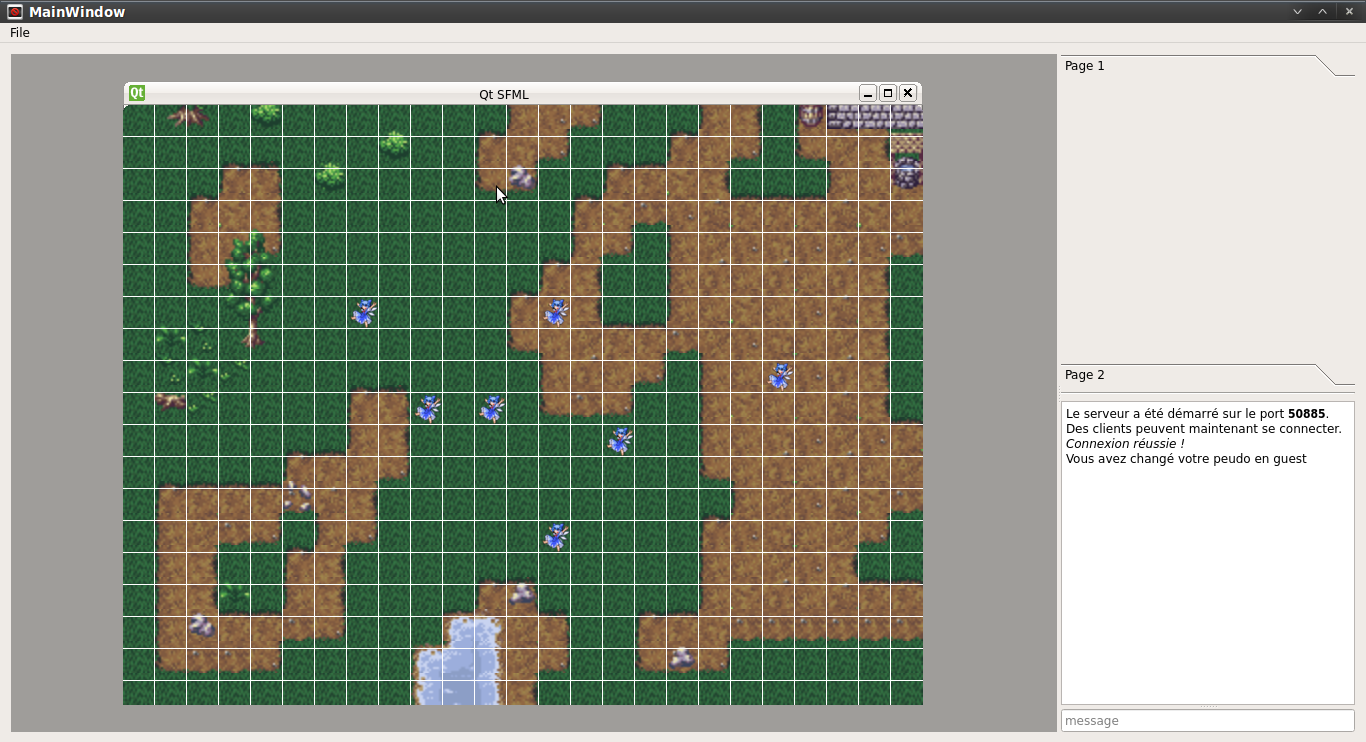
\includegraphics[width=0.8\textwidth]{img/gui_history/2014_05_07_screen.png}
	\caption{Interface du 7 Mai 2014}
\end{figure}

\begin{figure}[h!]
	\centering
	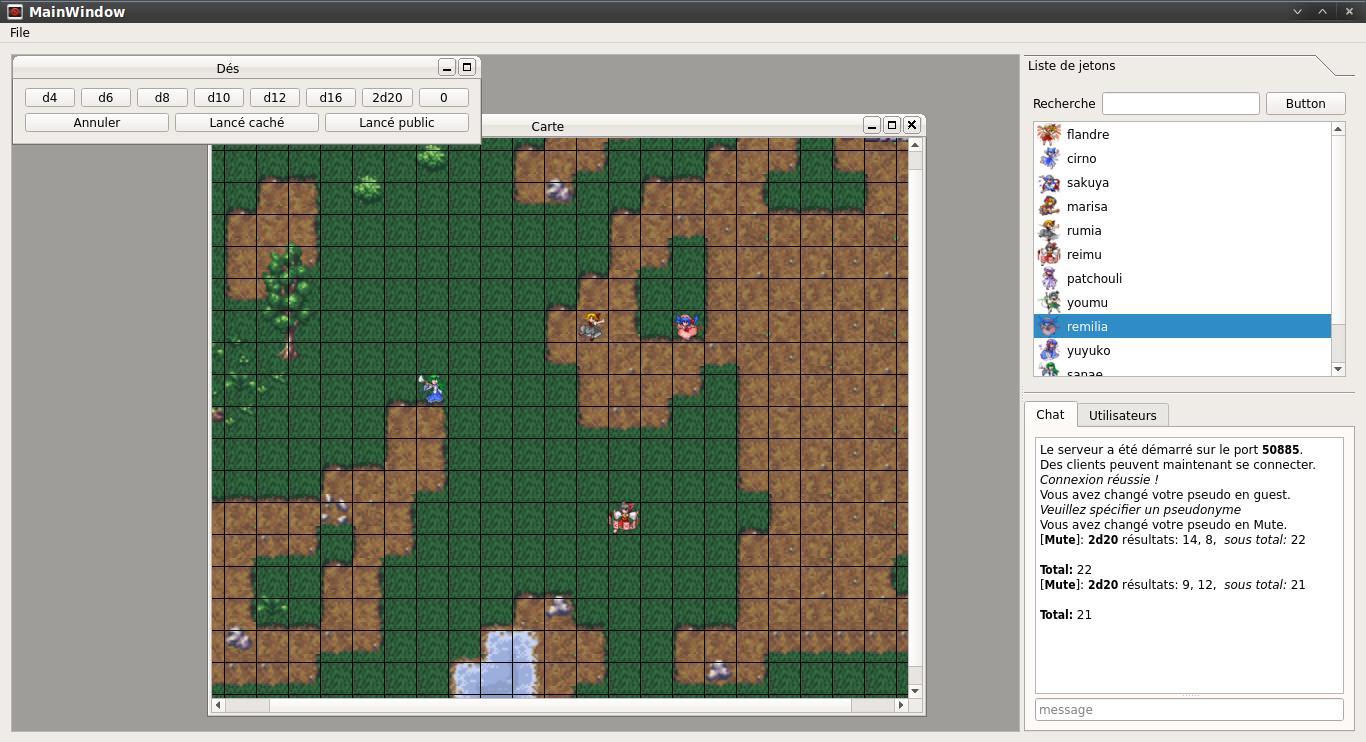
\includegraphics[width=0.8\textwidth]{img/gui_history/2014_05_21_screen.png}
	\caption{Interface du 21 Mai 2014 - Ajout des dés}
\end{figure}

\begin{figure}[h!]
	\centering
	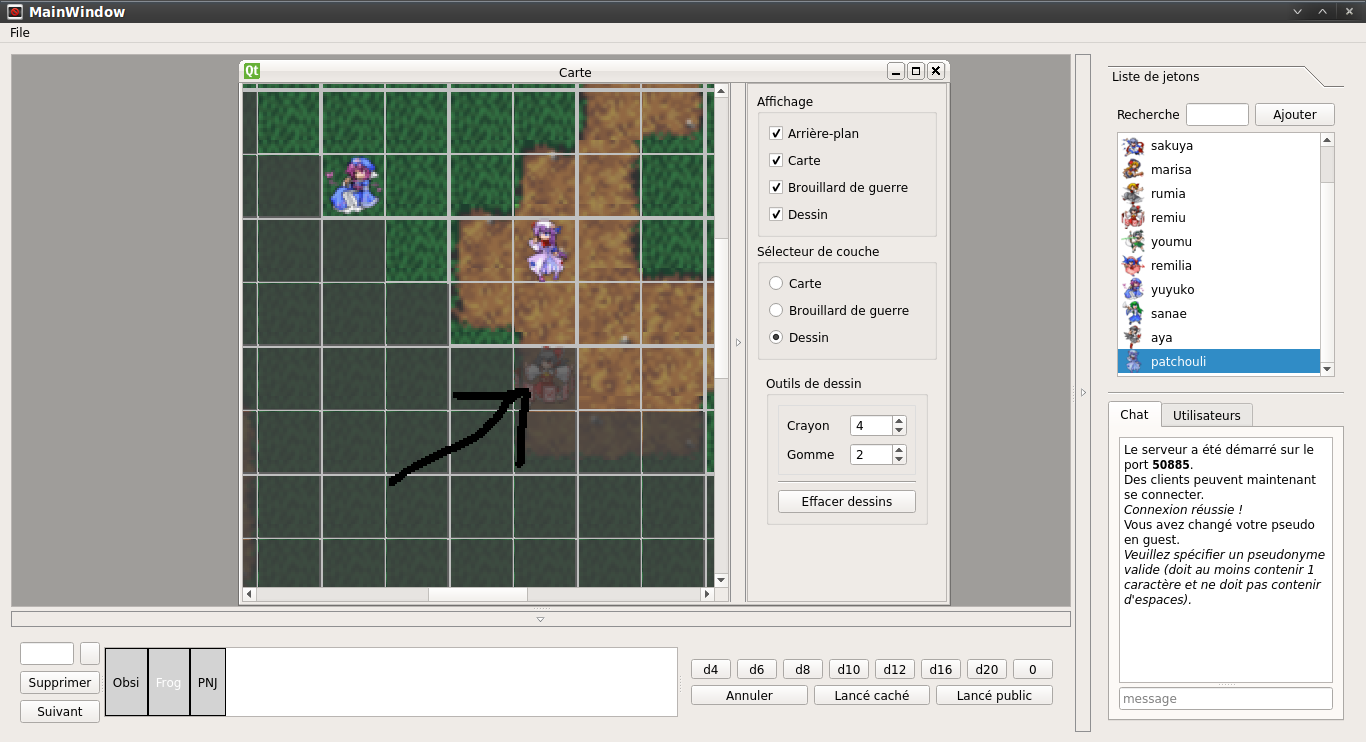
\includegraphics[width=0.8\textwidth]{img/gui_history/2014_05_30_screen.png}
	\caption{Interface du 30 Mai 2014 - Ajout du gestionnaire de tour + outils de carte}
\end{figure}

\begin{figure}[h!]
	\centering
	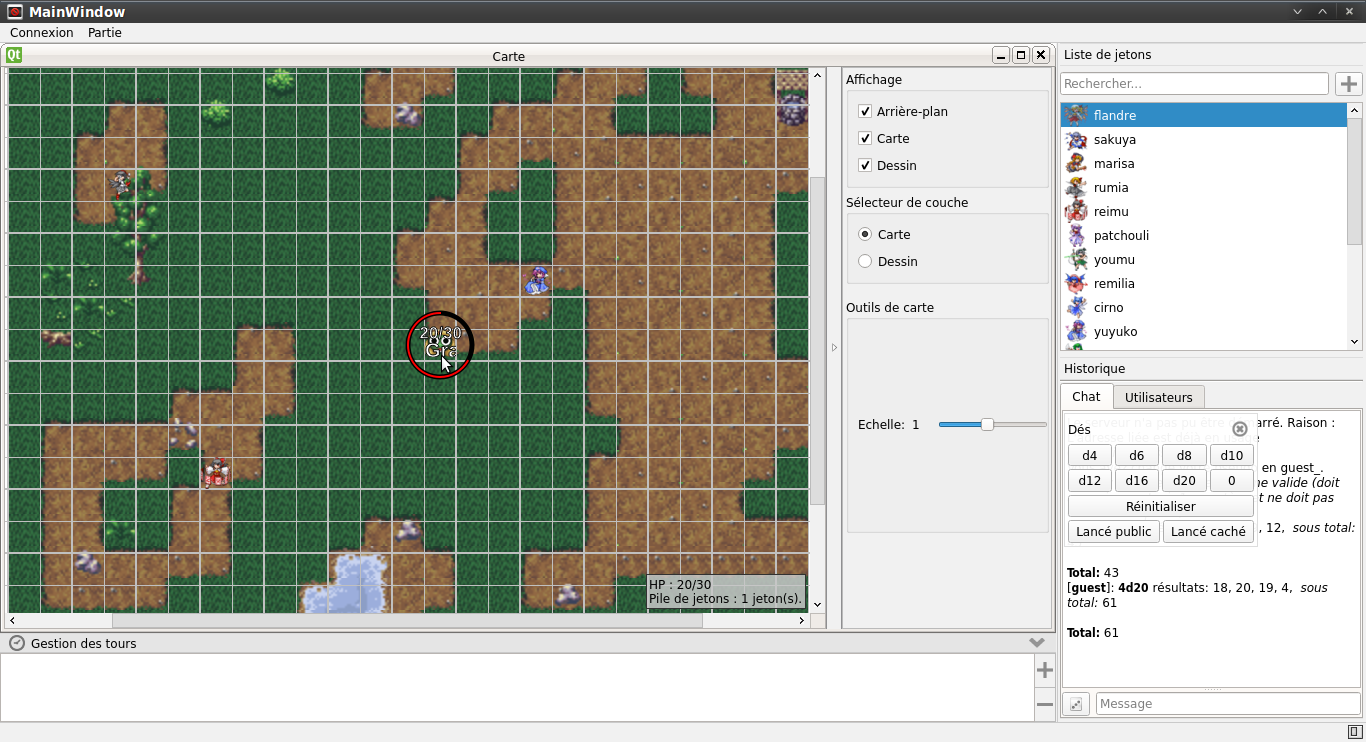
\includegraphics[width=0.8\textwidth]{img/gui_history/2014_06_18_screen.png}
	\caption{Interface du 18 Juin 2014 - Changement du style graphique}
\end{figure}

\section{Evolution technique}
\section{SFML}

Au début de notre projet, nous avions pensé à utiliser une bibliothèque graphique spécialisée dans la réalisation de jeu, SFML (\textit{Simple and Fast Multimedia Library}).\\

Cette bibliothèque nous aurait permis de réaliser facilement des animations et toute sorte d'effet graphique. 
Cependant, en utilisant SFML, de mauvaises réactions ont été constatées, notamment au niveau de l'affichage de la fenetre SFML.
Après plusieurs difficultés à faire cohabiter Qt et SFML, nous avons, au bout de deux semaines, nous avons décidé de réaliser l'application exclusivement avec Qt. Pour cela, nous avons dû repenser entièrement le système de carte déjà réalisé avec SFML.
